\section{Introduzione}

<<<<<<< HEAD
Il nostro progetto consiste nella realizzazione di un content-based recommender system che raccomandi film utilizzando dati provenienti dalla Linked Open Data Cloud al fine di poter aumentare l'efficienza del recommender system utilizzando informazioni aggiuntive inerenti un particolare film utilizzando differenti fonti.

\subsection{Linked Data}
L’interoperabilità è uno dei vantaggi più importanti del modello Open Data. I dati, se isolati, hanno poco valore; viceversa, il loro valore aumenta sensibilmente quando data set differenti, prodotti e pubblicati in modo indipendente da diversi soggetti, possono essere incrociati liberamente da terze parti. Questo è alla base del processo di creazione di valore aggiunto sui dati: le applicazioni. Le applicazioni, di valore sociale e/o economico, sfruttano quello che può essere visto come un grande database aperto e distribuito per offrire viste e servizi. L’interoperabilità è dunque un elemento chiave di uno degli aspetti più innovativi offerti dagli open data: l’uso dei dati in modi e per scopi “inattesi”, nuovi in quanto non previsti dai singoli enti e soggetti che pubblicano i “dati grezzi”.

Per consentire il riuso dei dati occorre poter combinare e mescolare liberamente i dataset. Occorre cioè collegare i dati tra loro, stabilendo un link diretto quando i dati (possibilmente provenienti da diverse sorgenti) si riferiscono a oggetti identici o comunque relazionati tra loro. Tale collegamento diretto si manifesta come la possibilità di “saltare” da un dataset all’altro, ad esempio quando si vuole accedere a dati (come i dettagli su una particolare entità) che non si posseggono al’interno.
Supponiamo per esempio di avere, da una parte, amministrazioni locali che pubblicano dati aperti relativi ai monumenti storici e agli hotel che si trovano nelle vicinanze di quei monumenti; dall’altra, Sovrintendenze ai Beni Culturali che pubblicano dati dettagliati sui monumenti, gli artisti e i periodi storici, e sui quadri esposti nei musei o nei palazzi.
Combinare i due dataset potrebbe essere di grande utilità, ad esempio per offrire un servizio personalizzato sugli itinerari in base agli interessi culturali specifici di un turista.
Per fare questo, se i dati non sono “collegati” (linked) occorre in qualche modo creare questi link, processando i dati a mano o attraverso algoritmi ad hoc. Questo processo può non essere banale e sicuramente è una barriera al riuso organico dei dati.

Nei cosiddetti Linked Data, questi collegamenti e relazioni tra le entità descritte nei dataset sono espliciti.
\subsection{Machine readable vs. machine linkable}
I linked data, per definizione, vengono espressi tramite Resource Description Framework (RDF). RDF non è propriamente un formato di dati, ma un “data model”, cioè un formalismo per rappresentare dati. Un dataset RDF può essere infatti serializzato in diversi formati (RDF/XML, N3, NTriple, etc.), ma il data model RDF possiede alcune caratteristiche che restano immutate, a prescindere dal formato che viene utilizzato.

In poche parole il modello RDF è costituito da triple, della forma soggetto-predicato-oggetto. Le triple possono condividere oggetto o soggetto così da formare un grafo.

\begin{figure}[htbp]
  \centering
  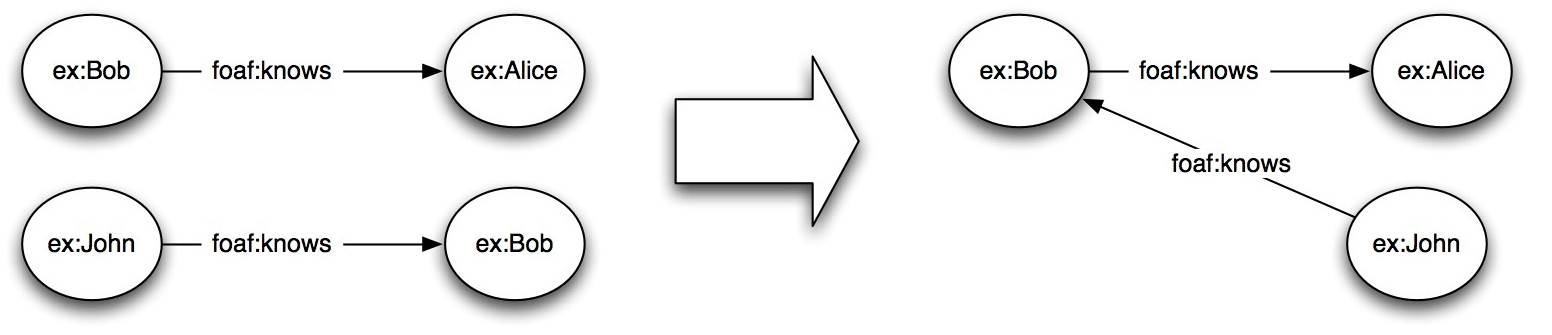
\includegraphics[width=.9\textwidth]
    {./images/triples1-crop}
\end{figure}

Questo insieme di triple RDF (o grafo) può essere espresso, allo scopo di essere scambiato tra applicazioni e pubblicato sul web, in vari formati di serializzazione.

Ad esempio in RDF/XML:
\lstset{ basicstyle=\LSTfont, columns=fullflexible, xleftmargin=5mm, framexleftmargin=5mm, numbers=left, stepnumber=1, breaklines=true, breakatwhitespace=false, numberstyle=\footnotesize, numbersep=5pt, tabsize=2, frame=lines, captionpos=b}
\begin{lstlisting}
<?xml version="1.0"?>
<rdf:RDF
    xmlns:ex="http://example.org/"
    xmlns:foaf="http://xmlns.com/foaf/0.1//"
    xmlns:rdf="http://www.w3.org/1999/02/22-rdf-syntax-ns#">
    <rdf:Description rdf:about="http://example.org/John">
        <foaf:knows>
            <rdf:Description rdf:about="http://example.org/Bob">
                <foaf:knows rdf:resource="http://example.org/Alice" />
            </rdf:Description>
        </foaf:knows>
    </rdf:Description>
</rdf:RDF>
\end{lstlisting}
La caratteristica più importante di tale modello, che si sposa con la visione Linked Data, è usare Uniform Resource Identifier (URI).


=======
Il nostro progetto consiste nella realizzazione di un content-based recommender system che raccomanda film che utilizza i dati provenienti dalla Linked Open Data Cloud per hsdfbjsdhvfhfbsdjfhbsdufh
>>>>>>> 1fd4b5df4f925cfacb4e9dc25651d223388c19b3
